%%%%%%%%%%%%%%%%%%%% author.tex %%%%%%%%%%%%%%%%%%%%%%%%%%%%%%%%%%%
%
% sample root file for your "contribution" to a contributed volume
%
% Use this file as a template for your own input.
%
%%%%%%%%%%%%%%%% Springer %%%%%%%%%%%%%%%%%%%%%%%%%%%%%%%%%%


% RECOMMENDED %%%%%%%%%%%%%%%%%%%%%%%%%%%%%%%%%%%%%%%%%%%%%%%%%%%
\documentclass[graybox]{svmult}

\usepackage[utf8]{inputenc}

% choose options for [] as required from the list
% in the Reference Guide

\usepackage{type1cm}        % activate if the above 3 fonts are
                            % not available on your system
%
\usepackage{makeidx}         % allows index generation
\usepackage{graphicx}        % standard LaTeX graphics tool
                             % when including figure files
\usepackage{multicol}        % used for the two-column index
\usepackage[bottom]{footmisc}% places footnotes at page bottom


\usepackage{newtxtext}       % 
\usepackage{newtxmath}       % selects Times Roman as basic font

% see the list of further useful packages
% in the Reference Guide

\makeindex             % used for the subject index
                       % please use the style svind.ist with
                       % your makeindex program

%%%%%%%%%%%%%%%%%%%%%%%%%%%%%%%%%%%%%%%%%%%%%%%%%%%%%%%%%%%%%%%%%%%%%%%%%%%%%%%%%%%%%%%%%

\begin{document}

\title*{Concept Reduction Methods}
% Use \titlerunning{Short Title} for an abbreviated version of
% your contribution title if the original one is too long
\author{Miklós F. Hatwagner}
% Use \authorrunning{Short Title} for an abbreviated version of
% your contribution title if the original one is too long
\institute{Miklós F. Hatwagner \at Széchenyi István University, Győr, Hungary \email{miklos.hatwagner@sze.hu}}
%
% Use the package "url.sty" to avoid
% problems with special characters
% used in your e-mail or web address
%
\maketitle

\abstract*{<To be prepared>}

\abstract{<To be prepared>}

\section{The Motivating Problem}
\label{sec:1}

The title of Adrienn Buruzs's PhD thesis \cite{buruzsphd2015} is ``Evaluation of Sustainable Regional Waste Management Systems with Fuzzy Cognitive Map''. As the title suggests, she analyzed the internal driving forces, dynamic behavior and sustainability of Integrated Waste Management Systems (IWMSs), which are very complex systems including many aspects (environmental, economic, social, institutional, legal and technical) and stakeholders. Even at an early stage of her investigations became apparent that Fuzzy Cognitive Map (FCM) is an appropriate tool to describe the large number of interacting and coupled entities and it copes with the inherent uncertainties of the system.

At first, a new FCM model \cite{buruzs2013developing} was created, which contained six concepts. These concepts were identified on the basis of the literature. The strength of relationships among concepts were defined by the results of a survey filled out by 75 stakeholders. The simulation results provided by FCM were validated later in \cite{buruzs2013advanced}. Time series data were collected based on the relevant literature and it served as the input of a Bacterial Evolutionary Algorithm to learn the connection weights among the already specified concepts and parameter $\lambda$ of the threshold function. The goal of optimization was to find an FCM that generates as similar time series as possible. Unfortunately, a strong contradiction was explored between the models created by experts and machine learning.

In order to resolve the experienced problem the concepts of the original model were decomposed to further 4-7 sub-concepts according to the System-of-Systems approach, which led to a very detailed, completely new model of IWMS \cite{buruzs2013modeling}. A workshop was organized with the help of 12 stakeholders who decided the sub-concepts and their interconnections. The result of their work is a FCM containing 33 concepts in total (Fig.~\ref{fig:flower}). Unfortunately such an extremely complex model is often confusing for the experts (Fig.~\ref{fig:fcmbig}), and to work with them  may be very laborious. Note that the number of connections is a quadratic function of the number of concepts.

That is why, in general, the following approach is suggested to follow in practice: start with an obviously oversized model. Experts are often uncertain about the importance of system components thus it worth include all of them in the preliminary model. Then start reducing the model automatically, in an algorithmic way until the balance of model size and required accuracy is found. In the following sections several possible ways of model reduction is presented.

\begin{figure}[hbt]
  \begin{center}
    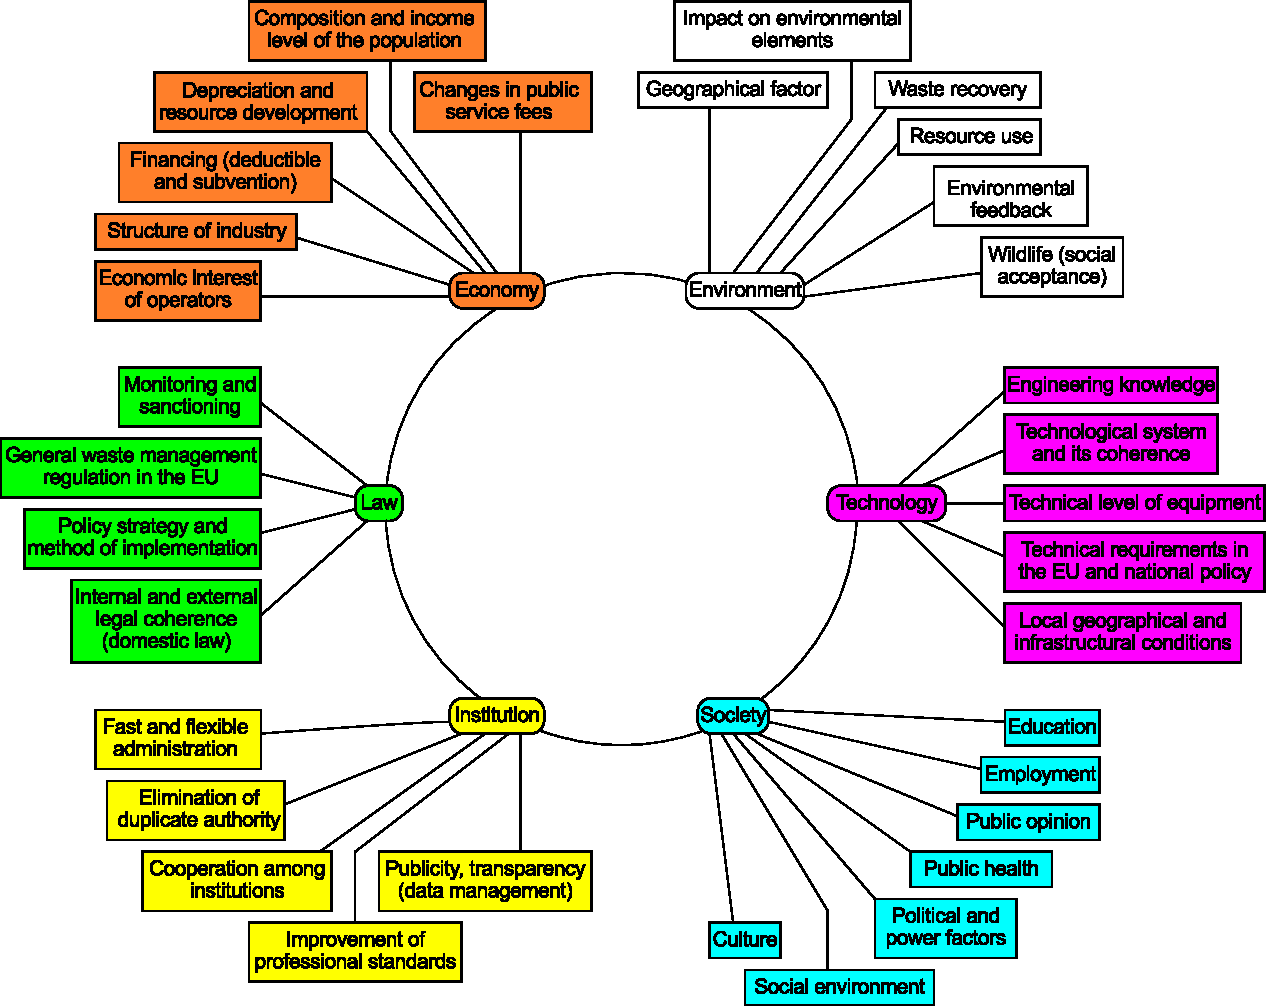
\includegraphics[width=\textwidth]{szines_virag.pdf}
  \end{center}
  \caption{The main concepts and their sub-concepts of regional IWMS.}
  \label{fig:flower}
\end{figure}

\begin{figure}[hbt]
  \begin{center}
    \includegraphics[width=\textwidth]{fcm_big.pdf}
  \end{center}
  \caption{The 33 concept model of regional IWMS and the relationships among its concepts. It is hard to illustrate complex FCM models appropriately and graphical model visualizations often confuse experts.}
  \label{fig:fcmbig}
\end{figure}

\section{Early model reduction methods}
\label{sec:2}

Several methods had been suggested to solve the problem of oversized models before the complex model of IWMS saw the light of the day. These approaches are based on different perspectives.

In \cite{alizadeh2008using} an FCM is learned using historical data and its concepts are grouped into clusters in a unique way. The clustering is based on the DEMATEL \cite{dematel} method. The concepts are arranged on a two dimensional plot. The vertical axis classifies concepts to cause and effect groups, the position of concepts along the horizontal axis expresses the importance of them. Based on this rearrangement of concepts two clustering methods are suggested. The first one uses K-Means clustering to create clusters according to the cause-effect behavior of concepts. The cluster centers replace the original concepts in the reduced model. The second method contains two consecutive steps, and takes also the importance of concepts into consideration. Regardless of the methods applied, experts have to define the number of clusters and they must be disjoint.

\begin{acknowledgement}
If you want to include acknowledgments of assistance and the like at the end of an individual chapter please use the \verb|acknowledgement| environment -- it will automatically be rendered in line with the preferred layout.
\end{acknowledgement}

%%%%%%%%%%%%%%%%%%%%%%%% referenc.tex %%%%%%%%%%%%%%%%%%%%%%%%%%%%%%
% sample references
% %
% Use this file as a template for your own input.
%
%%%%%%%%%%%%%%%%%%%%%%%% Springer-Verlag %%%%%%%%%%%%%%%%%%%%%%%%%%
%
% BibTeX users please use
\bibliographystyle{plain}
\bibliography{../hfmbibfile}
%
%\biblstarthook{References may be \textit{cited} in the text either by number (preferred) or by author/year.\footnote{Make sure that all references from the list are cited in the text. Those not cited should be moved to a separate \textit{Further Reading} section or chapter.} If the citatiion in the text is numbered, the reference list should be arranged in ascending order. If the citation in the text is author/year, the reference list should be \textit{sorted} alphabetically and if there are several works by the same author, the following order should be used:
%\begin{enumerate}
%\item all works by the author alone, ordered chronologically by year of publication
%\item all works by the author with a coauthor, ordered alphabetically by coauthor
%\item all works by the author with several coauthors, ordered chronologically by year of publication.
%\end{enumerate}
%The \textit{styling} of references\footnote{Always use the standard abbreviation of a journal's name according to the ISSN \textit{List of Title Word Abbreviations}, see \url{http://www.issn.org/en/node/344}} depends on the subject of your book:
%\begin{itemize}
%\item The \textit{two} recommended styles for references in books on \textit{mathematical, physical, statistical and computer sciences} are depicted in ~\cite{science-contrib, science-online, science-mono, science-journal, science-DOI} and ~\cite{phys-online, phys-mono, phys-journal, phys-DOI, phys-contrib}.
%\item Examples of the most commonly used reference style in books on \textit{Psychology, Social Sciences} are~\cite{psysoc-mono, psysoc-online,psysoc-journal, psysoc-contrib, psysoc-DOI}.
%\item Examples for references in books on \textit{Humanities, Linguistics, Philosophy} are~\cite{humlinphil-journal, humlinphil-contrib, humlinphil-mono, humlinphil-online, humlinphil-DOI}.
%\item Examples of the basic Springer Nature style used in publications on a wide range of subjects such as \textit{Computer Science, Economics, Engineering, Geosciences, Life Sciences, Medicine, Biomedicine} are ~\cite{basic-contrib, basic-online, basic-journal, basic-DOI, basic-mono}. 
%\end{itemize}
%}

%\begin{thebibliography}{99.}%
%% and use \bibitem to create references.
%%
%% Use the following syntax and markup for your references if 
%% the subject of your book is from the field 
%% "Mathematics, Physics, Statistics, Computer Science"
%%
%% Contribution 
%\bibitem{science-contrib} Broy, M.: Software engineering --- from auxiliary to key technologies. In: Broy, M., Dener, E. (eds.) Software Pioneers, pp. 10-13. Springer, Heidelberg (2002)
%%
%% Online Document
%\bibitem{science-online} Dod, J.: Effective substances. In: The Dictionary of Substances and Their Effects. Royal Society of Chemistry (1999) Available via DIALOG. \\
%\url{http://www.rsc.org/dose/title of subordinate document. Cited 15 Jan 1999}
%%
%% Monograph
%\bibitem{science-mono} Geddes, K.O., Czapor, S.R., Labahn, G.: Algorithms for Computer Algebra. Kluwer, Boston (1992) 
%%
%% Journal article
%\bibitem{science-journal} Hamburger, C.: Quasimonotonicity, regularity and duality for nonlinear systems of partial differential equations. Ann. Mat. Pura. Appl. \textbf{169}, 321--354 (1995)
%%
%% Journal article by DOI
%\bibitem{science-DOI} Slifka, M.K., Whitton, J.L.: Clinical implications of dysregulated cytokine production. J. Mol. Med. (2000) doi: 10.1007/s001090000086 
%%
%\bigskip

%% Use the following (APS) syntax and markup for your references if 
%% the subject of your book is from the field 
%% "Mathematics, Physics, Statistics, Computer Science"
%%
%% Online Document
%\bibitem{phys-online} J. Dod, in \textit{The Dictionary of Substances and Their Effects}, Royal Society of Chemistry. (Available via DIALOG, 1999), 
%\url{http://www.rsc.org/dose/title of subordinate document. Cited 15 Jan 1999}
%%
%% Monograph
%\bibitem{phys-mono} H. Ibach, H. L\"uth, \textit{Solid-State Physics}, 2nd edn. (Springer, New York, 1996), pp. 45-56 
%%
%% Journal article
%\bibitem{phys-journal} S. Preuss, A. Demchuk Jr., M. Stuke, Appl. Phys. A \textbf{61}
%%
%% Journal article by DOI
%\bibitem{phys-DOI} M.K. Slifka, J.L. Whitton, J. Mol. Med., doi: 10.1007/s001090000086
%%
%% Contribution 
%\bibitem{phys-contrib} S.E. Smith, in \textit{Neuromuscular Junction}, ed. by E. Zaimis. Handbook of Experimental Pharmacology, vol 42 (Springer, Heidelberg, 1976), p. 593
%%
%\bigskip
%%
%% Use the following syntax and markup for your references if 
%% the subject of your book is from the field 
%% "Psychology, Social Sciences"
%%
%%
%% Monograph
%\bibitem{psysoc-mono} Calfee, R.~C., \& Valencia, R.~R. (1991). \textit{APA guide to preparing manuscripts for journal publication.} Washington, DC: American Psychological Association.
%%
%% Online Document
%\bibitem{psysoc-online} Dod, J. (1999). Effective substances. In: The dictionary of substances and their effects. Royal Society of Chemistry. Available via DIALOG. \\
%\url{http://www.rsc.org/dose/Effective substances.} Cited 15 Jan 1999.
%%
%% Journal article
%\bibitem{psysoc-journal} Harris, M., Karper, E., Stacks, G., Hoffman, D., DeNiro, R., Cruz, P., et al. (2001). Writing labs and the Hollywood connection. \textit{J Film} Writing, 44(3), 213--245.
%%
%% Contribution 
%\bibitem{psysoc-contrib} O'Neil, J.~M., \& Egan, J. (1992). Men's and women's gender role journeys: Metaphor for healing, transition, and transformation. In B.~R. Wainrig (Ed.), \textit{Gender issues across the life cycle} (pp. 107--123). New York: Springer.
%%
%% Journal article by DOI
%\bibitem{psysoc-DOI}Kreger, M., Brindis, C.D., Manuel, D.M., Sassoubre, L. (2007). Lessons learned in systems change initiatives: benchmarks and indicators. \textit{American Journal of Community Psychology}, doi: 10.1007/s10464-007-9108-14.
%%
%%
%% Use the following syntax and markup for your references if 
%% the subject of your book is from the field 
%% "Humanities, Linguistics, Philosophy"
%%
%\bigskip
%%
%% Journal article
%\bibitem{humlinphil-journal} Alber John, Daniel C. O'Connell, and Sabine Kowal. 2002. Personal perspective in TV interviews. \textit{Pragmatics} 12:257--271
%%
%% Contribution 
%\bibitem{humlinphil-contrib} Cameron, Deborah. 1997. Theoretical debates in feminist linguistics: Questions of sex and gender. In \textit{Gender and discourse}, ed. Ruth Wodak, 99--119. London: Sage Publications.
%%
%% Monograph
%\bibitem{humlinphil-mono} Cameron, Deborah. 1985. \textit{Feminism and linguistic theory.} New York: St. Martin's Press.
%%
%% Online Document
%\bibitem{humlinphil-online} Dod, Jake. 1999. Effective substances. In: The dictionary of substances and their effects. Royal Society of Chemistry. Available via DIALOG. \\
%http://www.rsc.org/dose/title of subordinate document. Cited 15 Jan 1999
%%
%% Journal article by DOI
%\bibitem{humlinphil-DOI} Suleiman, Camelia, Daniel C. O'Connell, and Sabine Kowal. 2002. `If you and I, if we, in this later day, lose that sacred fire...': Perspective in political interviews. \textit{Journal of Psycholinguistic Research}. doi: 10.1023/A:1015592129296.
%%
%%
%%
%\bigskip
%%
%%
%% Use the following syntax and markup for your references if 
%% the subject of your book is from the field 
%% "Computer Science, Economics, Engineering, Geosciences, Life Sciences"
%%
%%
%% Contribution 
%\bibitem{basic-contrib} Brown B, Aaron M (2001) The politics of nature. In: Smith J (ed) The rise of modern genomics, 3rd edn. Wiley, New York 
%%
%% Online Document
%\bibitem{basic-online} Dod J (1999) Effective Substances. In: The dictionary of substances and their effects. Royal Society of Chemistry. Available via DIALOG. \\
%\url{http://www.rsc.org/dose/title of subordinate document. Cited 15 Jan 1999}
%%
%% Journal article by DOI
%\bibitem{basic-DOI} Slifka MK, Whitton JL (2000) Clinical implications of dysregulated cytokine production. J Mol Med, doi: 10.1007/s001090000086
%%
%% Journal article
%\bibitem{basic-journal} Smith J, Jones M Jr, Houghton L et al (1999) Future of health insurance. N Engl J Med 965:325--329
%%
%% Monograph
%\bibitem{basic-mono} South J, Blass B (2001) The future of modern genomics. Blackwell, London 
%%
%\end{thebibliography}

\end{document}
